\begin{frame}{Posterior Inference with MCMC}
\textbf{Algorithm:} sequential scan Metropolis-Hastings -- we visit each component of the parameters in turn, and for each component $j$ in iteration $t$, we propose
$$
X_{j} \sim q_{j}(\cdot \mid X_{1}^{(t)}, \ldots, X_{j-1}^{(t)}, X_{j}^{(t-1)}, \ldots, X_{d}^{(t-1)})
$$

\begin{itemize}
\vspace{0.2cm}
\item \textbf{Symmetric proposal $q_{j}$:} The proposal density cancels when evaluating the acceptance probability, and we are only left with the likelihood ratio (random Walk Metropolis-Hastings).
\vspace{0.2cm}
\item For each run, we simulate a Markov chain of length $100,000$ and select a sub-sample for every $100$ steps.
\vspace{0.2cm}
\end{itemize}
\end{frame}

\begin{frame}{MCMC Output Diagnostics -- Trace Plots}
\vspace{0.2cm}
\begin{itemize}
\item \textbf{Trace Plots:} stationary from the beginning of the simulation, suggesting that no burn-in period is required and we can keep the entire chain.
\end{itemize}

\begin{figure}
\centering
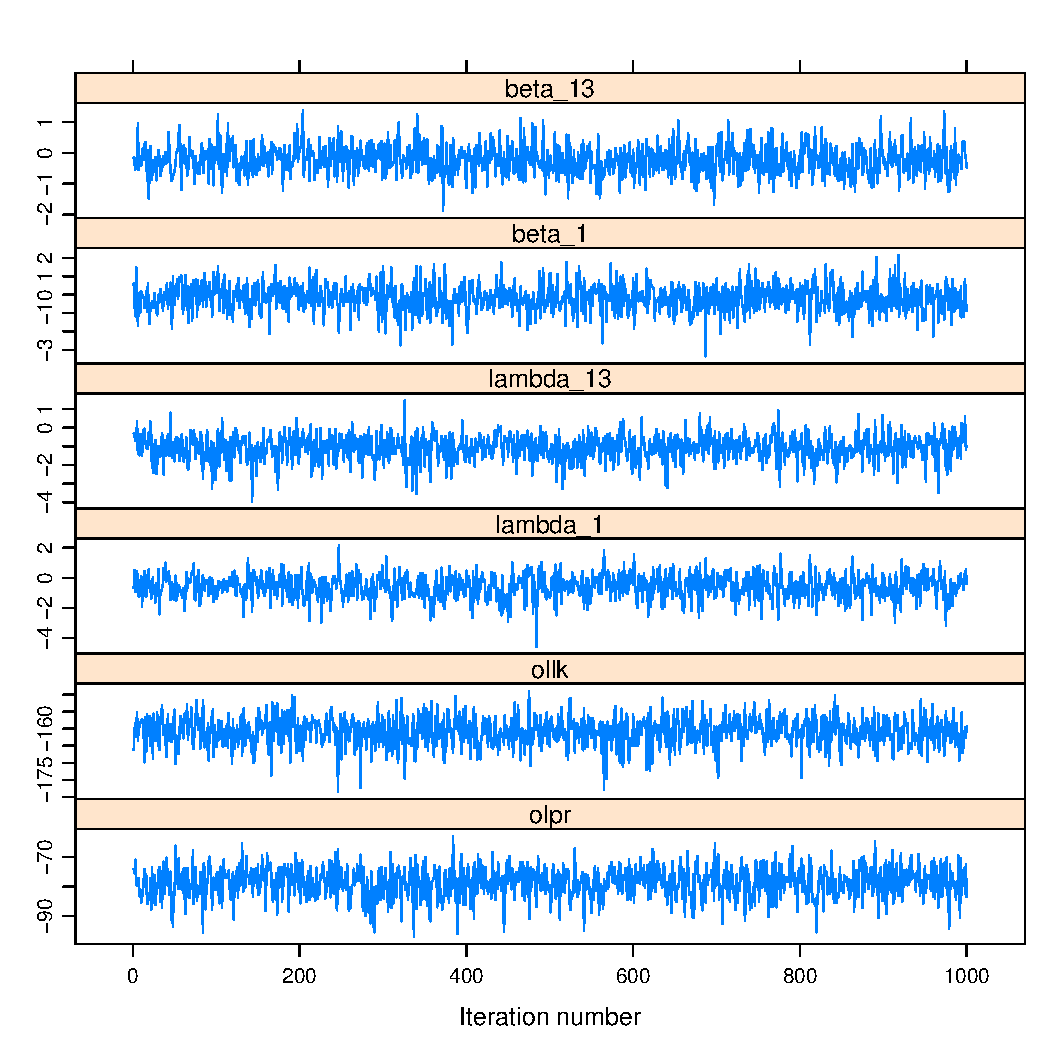
\includegraphics[width=.45\linewidth]{img/xyplot.pdf}
\caption{Trace plots of $\lambda^{(t)}, \beta^{(t)}$, the log-likelihood, and the log-prior}
\label{fig:xyplot}
\end{figure}
\end{frame}


\begin{frame}{MCMC Output Diagnostics -- Autocorrelations of Traces}
\vspace{0.2cm}
\begin{itemize}
\item \textbf{Autocorrelations of Traces:} fall off to zero quickly, so the effective sample size is close to the number of sub-samples 1000.
\end{itemize}

\begin{figure}
\centering
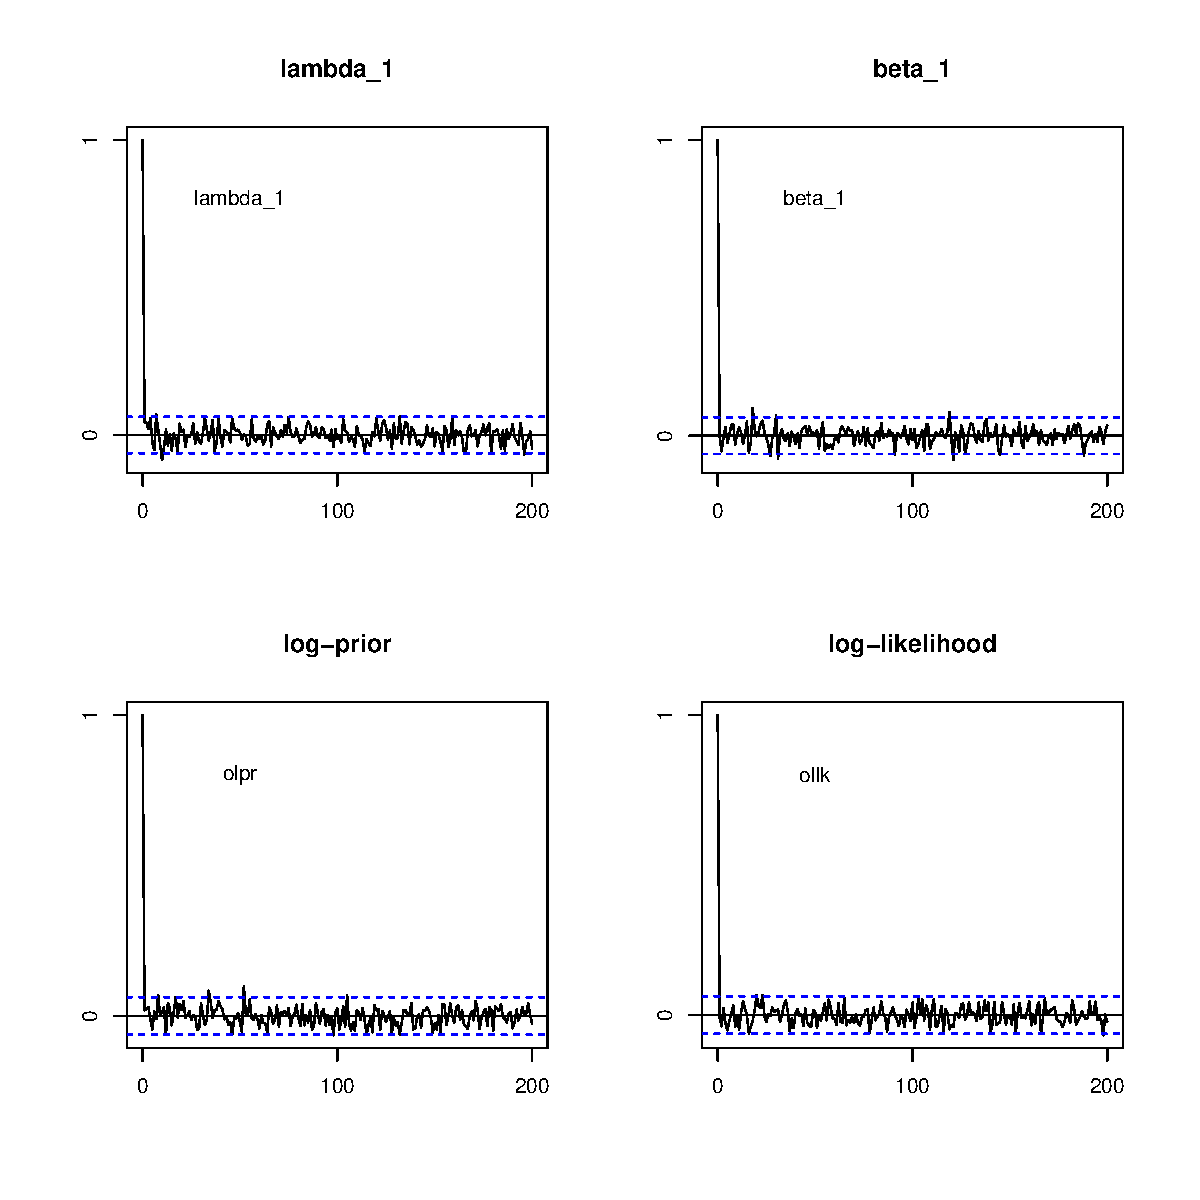
\includegraphics[width=.5\linewidth]{img/acf.pdf}
\caption{ACFs of the trace plots fall off to zero quickly}
\label{fig:acf}
\end{figure}
\end{frame}

\begin{frame}{MCMC Output Diagnostics -- Marginal Distributions}
\begin{itemize}
\item \textbf{Marginal Distributions:} perform multiple runs from different start states and check those marginal agree
\vspace{0.2cm}
\end{itemize}

\begin{figure}
\centering
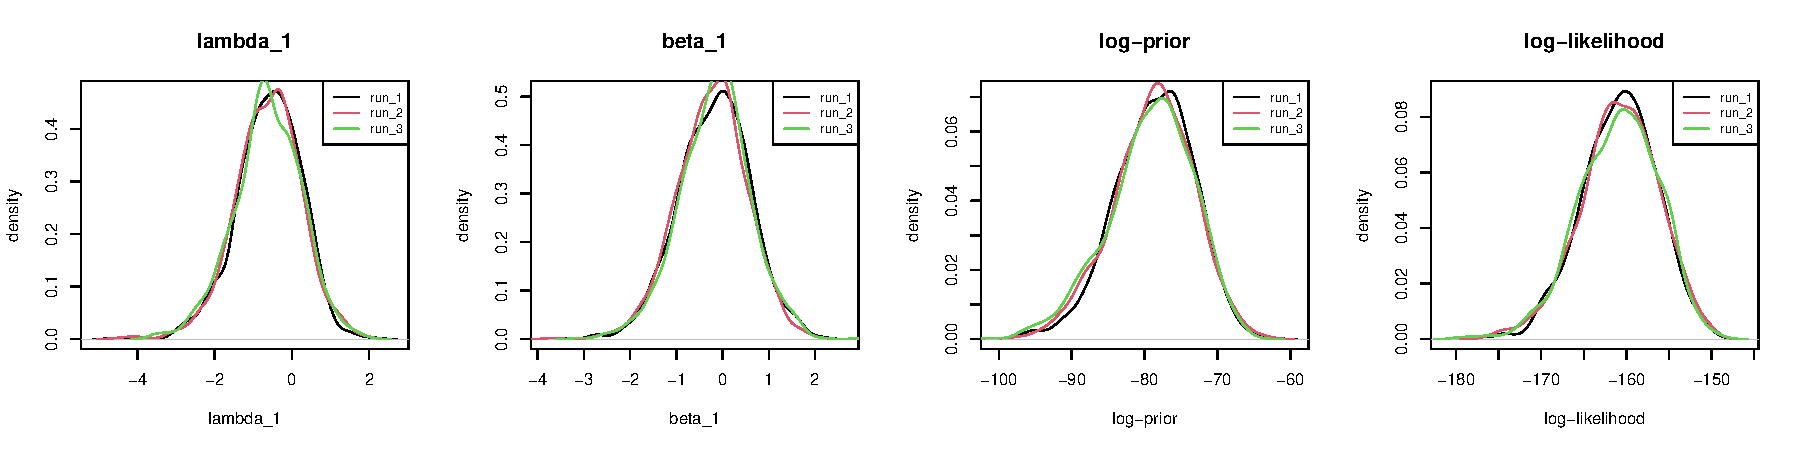
\includegraphics[width=\linewidth]{img/runs.pdf}
\caption{Density plots of the variables and key functions in three runs with different start states}
\label{fig:runs}
\end{figure}

From the diagnostic plots:
\vspace{0.2cm}
\begin{itemize}
\item Good convergence of the chain to the target distribution
\item Good explorations of the parameter space of the target posterior
\end{itemize}
\end{frame}

\begin{frame}{Player Skills}
From the posterior mean, we can conclude that players $21,19,4$ have the strongest skills, whereas players $20,2,9$ have the weakest.
\begin{table} \center
\begin{tabular}{cccc}
\text { Param. } & \text { Post. Mean } & \text {95\% HPD interval } & \text { ESS } \\
\hline
$\lambda_{1}$ & -0.67 & (-2.18, 0.85) & 1132 \\
$\lambda_{2}$ & -2.31 & (-4.09, -0.44) & 884 \\
$\lambda_{3}$ & -1.35 & (-3.68, 0.52) & 1000 \\
$\lambda_{4}$ & 1.35 & (-0.11, 2.97) & 1000 \\
$\lambda_{5}$ & -0.45 & (-1.41, 0.42) & 1000 \\
$\lambda_{6}$ & -0.11 & (-1.75, 1.50) & 1000 \\
$\lambda_{7}$ & 0.76 & (0.07, 1.51) & 1000 \\
$\lambda_{8}$ & 0.30 & (-0.54, 1.13) & 1230 \\
$\lambda_{9}$ & -2.25 & (-3.58, -1.01) & 1000 \\
$\lambda_{10}$ & 0.39 & (-0.19, 1.05) & 1000 \\
$\lambda_{11}$ & 0.20 & (-0.51, 0.94) & 1000 \\
$\lambda_{12}$ & 0.90 & (-0.26, 1.81) & 1000 \\
$\lambda_{13}$ & -0.82 & (-2.08, 0.45) & 960 \\
\end{tabular}
\end{table}
\end{frame}

\begin{frame}{Player Skills}
\begin{table} \center
\begin{tabular}{cccc}
\text { Param. } & \text { Post. Mean } & \text {95\% HPD interval} & \text { ESS } \\
\hline
$\lambda_{14}$ & 0.09 & (-1.15, 1.44) & 1000 \\
$\lambda_{15}$ & -0.26 & (-1.07, 0.40) & 1000 \\
$\lambda_{16}$ & 1.17 & (-0.23, 2.56) & 1000 \\
$\lambda_{17}$ & 0.91 & (-0.28, 2.04) & 1077 \\
$\lambda_{18}$ & -1.44 & (-3.41, 0.05) & 798 \\
$\lambda_{19}$ & 2.03 & (0.79, 3.36) & 1000 \\
$\lambda_{20}$ & -2.36 & (-4.57, -0.57) & 825 \\
$\lambda_{21}$ & 2.91 & (0.23, 6.02) & 879 \\
$\lambda_{22}$ & -0.19 & (-1.84, 1.44) & 1000 \\
$\lambda_{23}$ & -0.97 & (-3.05, 1.26) & 1000 \\
$\lambda_{24}$ & 0.81 & (-0.42, 2.12) & 1000 \\
$olpr$ & -44.39 & (-52.62, -36.49) & 1000 \\
$ollk$ & -161.1 & (-168.27, -153.29) & 1000 \\
\end{tabular}
\caption{Summary of the posterior mean, HPD intervals and the ESS}
\end{table}
\end{frame}

\begin{frame}{Player Skills}
\vspace{0.2cm}
Perform a comparison of the relative skills of each pair $\{i, j\}$ of players by considering games involving only the two players
$$
\operatorname{Pr}\{i \operatorname{win}\}=\frac{\exp \left(\hat{\lambda}_{o_i}\right)}{\exp \left(\hat{\lambda}_{o_i}\right)+\exp \left(\hat{\lambda}_{o_j}\right)}
$$
\begin{figure}
\centering
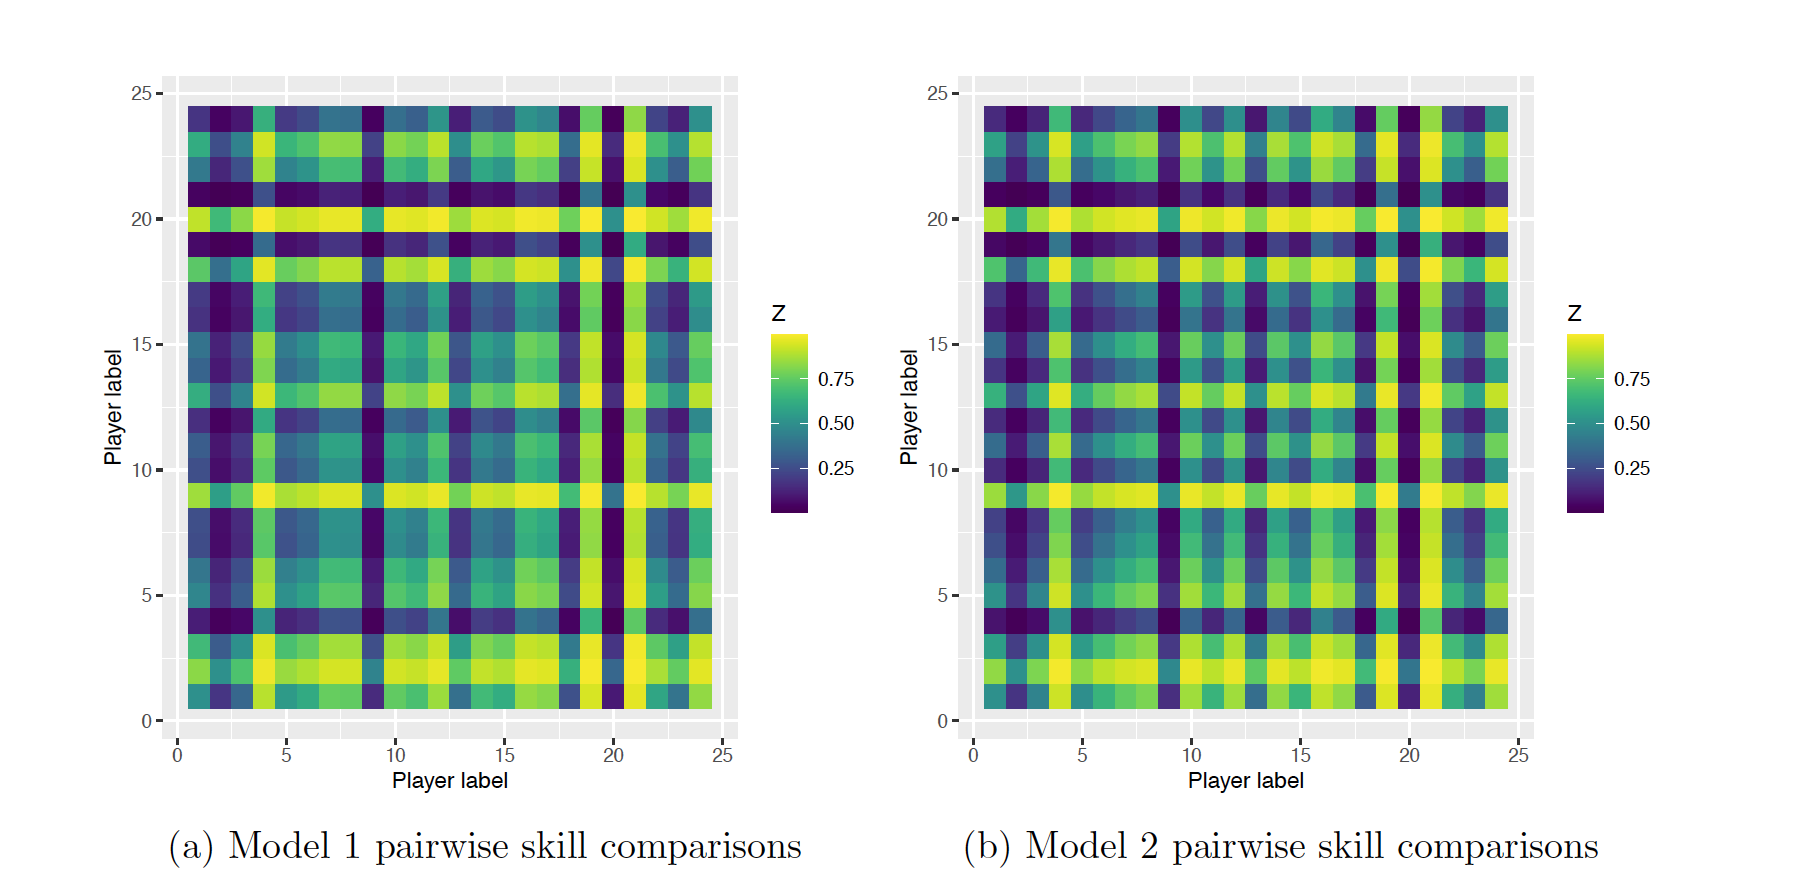
\includegraphics[width=0.84\linewidth]{img/heat.png}
\caption{Pairwise comparisons of the relative skills of the players}
\label{fig:heat}
\end{figure}
\end{frame}

\begin{frame}{Model selection}
We use the Bayes factor $B_{1,2}$ to perform a model comparison between Model 1 (without seniority) and Model 2 (with seniority)
$$
B_{1,2}=\frac{p\left(y \mid m=1\right)}{p\left(y \mid m=2\right)}=\frac{\int p\left(y \mid \theta, m=1\right) \pi_{m=1}(\theta) d \theta}{\int p(y \mid \theta, m=2) \pi_{m=2}(\theta) d \theta}
$$

\begin{itemize}
\item Compute the marginal $p(y \mid m)$ using the Bridge estimator
$$
\widehat{p}=\frac{\sum_t \pi\left(\theta^{(1, t)}\right) p\left(y \mid \theta^{(1, t)}\right) h\left(\theta^{(1, t)}\right)}{\sum_t \pi\left(\theta^{(2, t)}\right) h\left(\theta^{(2, t)}\right)}
$$
\item Choose $h(\theta)=\pi(\theta)^{-1} p(y \mid \theta)^{-1 / 2}$ that minimises the MSE
$$
\widehat{p}=\frac{\sum_t p\left(y \mid \theta^{(1, t)}\right)^{1 / 2}}{\sum_t p\left(y \mid \theta^{(2, t)}\right)^{-1 / 2}}
$$
\item $\theta^{(1, t)} \sim \pi(\theta)$ are random samples simulated from the prior
\item $\theta^{(2, t)} \sim \pi(\theta \mid y)$ are simulated from the posterior
\end{itemize}
\end{frame}

\begin{frame}{Model selection}
\textbf{Conclusion:} The estimated Bayes factor $\widehat{B}_{1,2}$ has the order of magnitude of $10^5$ and does not vary upon multiple computations, providing substantial evidence in favour of the model without seniority covariates than the model with.
\end{frame}

\begin{frame}{Interesting Counter Example}
Consider a simple example where game $68$ involving nine players $s=\{4, 7, 11, 5, 10, 14, 15, 13, 9\}$ was replayed (i.e. with the same players and same seniority values), we are interested in the probability that player $7$ wins. We estimate this by summing the probabilities of all $8!$ permutations where player $7$ comes at the top
\begin{equation*}
  \sum_{o_{1}=7} E_{\lambda, \beta \mid model} \left[ \operatorname{Pr}\{O=o \mid \lambda, \beta\} \right] \quad \text{where} \quad O \in \mathcal{P}_{s}
\end{equation*}

\begin{itemize}
\item The marginals are estimated using the Bridge estimator
\item In model one without seniority covariates, the probability is $17.4\%$
\item With model two, when the seniority covariates are added, the probability that player $7$ wins drops to $4.1\%$
\item Seniority has \textbf{non-trivial} effects on the outcomes
\end{itemize}
\end{frame}
